\documentclass[11pt]{article}

\usepackage[margin=1in]{geometry}
\usepackage{amsmath, amssymb, amsthm, bm}
\usepackage{booktabs}
\usepackage{graphicx}
\usepackage{hyperref}

\title{Sequential Tradeability Testing for Alpha Signals}
\author{Rany Stephan}
\date{\today}

\newtheorem{proposition}{Proposition}

\begin{document}
\maketitle

\begin{abstract}
Many candidate alpha signals have positive historical predictive content but fail after
uncertainty, decay, turnover, and market impact are considered.  This project studies
alpha validation as a sequential decision problem.  Starting from the Bayesian drift
estimation framework of Ekstrom, Karatzas, and Vaicenavicius, we model the evidence for
an alpha signal as a noisy observation process with an unknown drift.  The posterior mean
and posterior variance form the state variables, and the decision to continue observing,
activate, or retire the signal becomes an optimal stopping problem.  The first step of the
project derives and verifies the filtering identities that will later be extended with
transaction costs and alpha decay.
\end{abstract}

\section{Base Sequential Estimation Model}

Let \(X\) denote the unknown strength of a candidate alpha signal.  In the base model,
we observe a noisy evidence process
\begin{equation}
    Y_t = X t + W_t, \qquad t \ge 0,
    \label{eq:observation_model}
\end{equation}
where \(W\) is a standard Brownian motion independent of \(X\).  The prior distribution
of \(X\) is denoted by \(\mu\), and the observation filtration is
\[
    \mathcal F_t^Y = \sigma(Y_s:0\le s\le t).
\]
In the alpha interpretation, \(Y_t\) can be read as cumulative signal evidence, such as
cumulative signal-aligned residual return or cumulative information coefficient, after
appropriate normalization.

The least-squares estimate of \(X\) is the posterior mean
\begin{equation}
    \widehat X_t = \mathbb E[X\mid \mathcal F_t^Y].
\end{equation}
For any prior with finite second moment, Bayes' rule gives the posterior distribution
\begin{equation}
    \mu_{t,y}(du)
    =
    \frac{\exp\{uy-u^2t/2\}\mu(du)}
    {\int_{\mathbb R}\exp\{vy-v^2t/2\}\mu(dv)}.
    \label{eq:posterior}
\end{equation}
Thus the posterior mean and posterior variance are
\begin{align}
    G(t,y)
    &=
    \frac{\int_{\mathbb R}u\exp\{uy-u^2t/2\}\mu(du)}
    {\int_{\mathbb R}\exp\{uy-u^2t/2\}\mu(du)},\\
    H(t,y)
    &=
    \int_{\mathbb R}(u-G(t,y))^2\mu_{t,y}(du).
\end{align}
The estimate is therefore \(\widehat X_t=G(t,Y_t)\).

\section{Filtering Identity}

The innovation process is
\begin{equation}
    \widehat W_t
    =
    Y_t-\int_0^t \widehat X_s\,ds.
\end{equation}
It is a Brownian motion in the observation filtration.  If \(G_t(\cdot)=G(t,\cdot)\)
and
\begin{equation}
    \Psi(t,x) = H(t,G_t^{-1}(x)),
    \label{eq:psi_definition}
\end{equation}
then the posterior mean satisfies
\begin{equation}
    d\widehat X_t = \Psi(t,\widehat X_t)\,d\widehat W_t.
    \label{eq:posterior_mean_sde}
\end{equation}
The same function \(\Psi\) is also the conditional mean-squared error:
\begin{equation}
    \Psi(t,\widehat X_t)
    =
    \operatorname{Var}(X\mid \mathcal F_t^Y).
\end{equation}
This dual role is the mathematical reason the problem admits a clean stopping
formulation: posterior uncertainty is both the remaining estimation error and the local
volatility of the posterior mean.

\section{Optimal Stopping Interpretation}

Ekstrom, Karatzas, and Vaicenavicius study
\begin{equation}
    \inf_{\tau}
    \mathbb E\left[(X-\widehat X_\tau)^2+c\tau\right],
    \label{eq:ekv_objective}
\end{equation}
where \(c>0\) is the observation cost per unit time.  Since
\[
    \mathbb E[(X-\widehat X_\tau)^2]
    =
    \mathbb E[\Psi(\tau,\widehat X_\tau)],
\]
the objective can be written in posterior-variance form.

\begin{proposition}[EKV variance decay identity]
For any admissible stopping time \(\tau\),
\begin{equation}
    \mathbb E[\Psi(\tau,\widehat X_\tau)]
    =
    \operatorname{Var}(X)
    -
    \mathbb E\left[\int_0^\tau \Psi^2(s,\widehat X_s)\,ds\right].
    \label{eq:variance_decay_identity}
\end{equation}
\end{proposition}

Consequently, minimizing \eqref{eq:ekv_objective} is equivalent, up to the constant
\(\operatorname{Var}(X)\), to minimizing
\begin{equation}
    \inf_{\tau}
    \mathbb E\left[
    \int_0^\tau
    \left(c-\Psi^2(s,\widehat X_s)\right)ds
    \right].
    \label{eq:running_cost_form}
\end{equation}
The interpretation is direct: observing for one more instant costs \(c\), while the
instantaneous rate of posterior-variance reduction is \(\Psi^2\).  The continuation
region is therefore the set where the option value of further learning exceeds the
observation cost.

\section{Two Checkable Priors}

\subsection{Gaussian prior}

If \(X\sim N(m,\sigma^2)\), then
\begin{equation}
    \widehat X_t
    =
    \frac{m+\sigma^2Y_t}{1+\sigma^2t},
    \qquad
    \Psi(t,x)
    =
    \frac{\sigma^2}{1+\sigma^2t}.
\end{equation}
The posterior variance is deterministic.  The optimal stopping time is
\begin{equation}
    \tau^\star
    =
    \left(\frac{1}{\sqrt c}-\frac{1}{\sigma^2}\right)^+.
    \label{eq:gaussian_tau}
\end{equation}
This case will serve as our first validation benchmark: the code must reproduce the
precision update and the variance decay identity exactly.

\subsection{Symmetric Bernoulli prior}

If \(X\in\{-\beta,\beta\}\), then the posterior mean lies in \((-\beta,\beta)\) and
\begin{equation}
    \Psi(x)=\beta^2-x^2.
\end{equation}
When \(\beta^4\le c\), immediate stopping is optimal.  Otherwise the optimal stopping
time is the first exit from a symmetric interval:
\begin{equation}
    \tau_a^\star
    =
    \inf\{t\ge 0:|\widehat X_t|\ge a\},
\end{equation}
where \(a\in(\gamma,\beta)\), \(\gamma=\sqrt{\beta^2-\sqrt c}\), solves
\begin{equation}
    \int_0^a
    \frac{c-(\beta^2-\xi^2)^2}{(\beta^2-\xi^2)^2}\,d\xi
    =
    0.
    \label{eq:bernoulli_boundary}
\end{equation}
This case is the first mathematical template for alpha activation or rejection: continue
while the evidence is ambiguous, and stop once posterior confidence is sufficiently far
from zero.

\section{Project Translation}

The base paper estimates an unknown drift.  Our project will preserve the posterior
state and stopping-boundary structure, but change the terminal payoff from estimation
accuracy to economic tradeability.  The intended mapping is:
\[
\begin{array}{lll}
\text{EKV variable} & & \text{alpha tradeability variable}\\
\midrule
X && \text{unknown alpha strength}\\
Y_t && \text{cumulative normalized signal evidence}\\
\widehat X_t && \text{posterior mean alpha}\\
\Psi(t,\widehat X_t) && \text{posterior uncertainty and learning speed}\\
c && \text{observation, opportunity, and implementation cost}\\
\tau && \text{activation, rejection, or retirement time}.
\end{array}
\]
The next mathematical step is to define a finance terminal payoff
\(\Phi(m,q;\mathrm{cost})\) that rewards activation only when posterior alpha value
survives uncertainty and transaction costs.  Once that payoff is fixed, the project
becomes a numerically solvable optimal stopping problem whose boundary can be compared
against fixed \(t\)-statistic, rolling Sharpe, and IC-threshold rules.

\section{A First Tradeability Payoff}

We now define the first finance version of the terminal stopping payoff.  Suppose that,
at a stopping time, the posterior belief about the signal strength is summarized by mean
\(m\) and variance \(q\).  If the signal is activated with signed exposure \(z\), we use the
posterior predictive mean-variance objective
\begin{equation}
    m z
    -
    \frac{\lambda}{2}(\sigma_r^2+q)z^2
    -
    \kappa.
    \label{eq:activation_objective}
\end{equation}
Here \(\lambda>0\) is risk aversion, \(\sigma_r^2\) is the residual return variance of the
traded signal, \(q\) is posterior parameter uncertainty, and \(\kappa\ge 0\) is an
implementation hurdle representing spread, impact, research delay, or capital allocation
cost.  Optimizing \eqref{eq:activation_objective} over \(z\in\mathbb R\) gives
\begin{equation}
    \sup_z
    \left\{
    mz-\frac{\lambda}{2}(\sigma_r^2+q)z^2-\kappa
    \right\}
    =
    \frac{m^2}{2\lambda(\sigma_r^2+q)}-\kappa.
\end{equation}
Since the decision maker can reject the signal instead of trading it, the terminal payoff is
\begin{equation}
    \Phi(m,q)
    =
    \left(
    \frac{m^2}{2\lambda(\sigma_r^2+q)}
    -
    \kappa
    \right)^+.
    \label{eq:tradeability_payoff}
\end{equation}
The immediate activation threshold is therefore
\begin{equation}
    |m|
    >
    \sqrt{2\lambda(\sigma_r^2+q)\kappa}.
    \label{eq:activation_threshold}
\end{equation}
This is only a terminal threshold.  Before the final validation date, the signal also has
option value: a currently ambiguous signal may become tradeable after more evidence
arrives.

\section{Finite-Horizon Stopping Problem}

For the Gaussian prior, the posterior variance is deterministic:
\[
    q(t)=\frac{q_0}{1+q_0t},
\]
and the posterior mean follows
\begin{equation}
    dm_t = q(t)\,d\widehat W_t.
\end{equation}
Given a finite validation horizon \(T\), the tradeability value is
\begin{equation}
    V(t,m)
    =
    \sup_{\tau\in[t,T]}
    \mathbb E_{t,m}
    \left[
        e^{-\rho \tau}\Phi(m_\tau,q(\tau))
        -
        \int_t^\tau c\,ds
    \right].
    \label{eq:tradeability_value}
\end{equation}
The parameter \(\rho\ge 0\) captures alpha decay or opportunity loss during validation.
This term is economically important.  Without decay or discounting, the activation
payoff is convex in the posterior mean \(m\), and the model can prefer to keep observing
even when \(|m|\) is already very large.  That is the wrong lifecycle decision for a
decaying alpha: a sufficiently strong signal should be activated before its deployable
value evaporates.

The continuation region satisfies the variational inequality
\begin{equation}
    \max\left\{
        e^{-\rho t}\Phi(m,q(t))-V(t,m),
        \partial_t V(t,m)
        +
        \frac{1}{2}q(t)^2\partial_{mm}V(t,m)
        -
        c
    \right\}
    =
    0,
    \label{eq:tradeability_vi}
\end{equation}
with terminal condition
\begin{equation}
    V(T,m)=e^{-\rho T}\Phi(m,q(T)).
\end{equation}

This is the first paper-level object we can compute.  It has the right economic
interpretation:
\begin{itemize}
    \item high \(|m|\) favors stopping and activating the signal;
    \item low posterior variance \(q\) lowers the option value of more observation;
    \item high observation or implementation cost shrinks the continuation region;
    \item near \(m=0\), the payoff can be zero while continuation value remains positive,
    because future evidence may still move the posterior mean into the tradeable region.
\end{itemize}

The code solves \eqref{eq:tradeability_vi} by backward implicit Euler on a uniform grid in
\((t,m)\), with the mean-domain boundaries pinned to the immediate stopping payoff.  The
implementation is validated against exact activation thresholds, symmetry in \(m\), the
zero-payoff no-continuation case, monotonic decline of value as observation cost rises, and
early exercise of strong alpha when \(\rho>0\).

\begin{figure}[t]
    \centering
    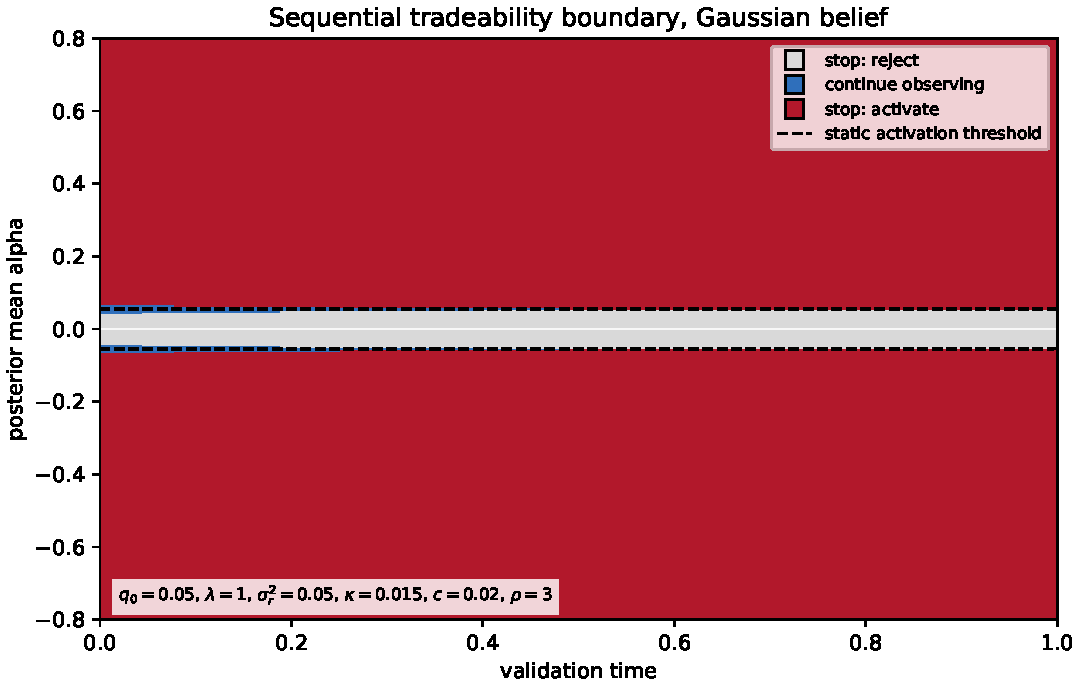
\includegraphics[width=0.92\linewidth]{../figures/gaussian_tradeability_boundary.pdf}
    \caption{First finite-difference tradeability boundary for the Gaussian-belief model.
    Red states stop and activate the alpha, gray states stop and reject it, and blue states
    continue observing.  The dashed curves show the static activation threshold from
    \eqref{eq:activation_threshold}; the dynamic boundary is wider because ambiguous
    signals have option value early in the validation period.}
    \label{fig:gaussian_tradeability_boundary}
\end{figure}

\end{document}
